\chapter{Methods}

\section{Theoretical Models}

Our model is based on the classic Wright-Fisher \cite{wright_evolution_1931}\cite{fisher_mathematical_1922} and Stepping Stone \cite{kimura_stepping_1964} population genetic models which describe evolution and migration, respectively. More precisely, our model represents Wrighht-Fisher evolutionary dynamics within a Stepping Stone migration framework. In this section, we present the logic of these models using the parameterization best suited for our purposes. Namely, we consider a \textit{haploid} population of size $N$ as opposed to a \textit{diploid} population. However, much of the following derivations are applicable to diploid models. The modified derivations largely follow the logic of the original Wright \cite{wright_evolution_1931} and Kimura \cite{kimura_stepping_1964} papers \cite{Rackauckas2014AnII}\cite{tran_introduction_2013} \cite{durrett_probability_2008}.


\subsection{The neutral Wright-Fisher model} \label{section:neutral_wf}

The neutral Wright-Fisher model \cite{wright_evolution_1931}\cite{fisher_mathematical_1922}, named after population geneticists Sewall Wright and Ronald Fisher, considers an idealized population with random mating, non-overlapping generation times; and without mutation, migration or natural selection. Despite these assumptions, the model serves as a useful tool for studying evolutionary forces acting upon a population, particularly genetic drift. More complex evolutionary forces can be incorporated seamlessly, as our work will show. 


We start by considering a \textit{haploid} population of finite size $N$ and a single genetic locus with two alleles, $A$ and $a$. The total population size remains constant. Let $X_t$ be the number of $A$ alleles at generation $t$.Therefore, the frequency of $A$, $f_t$, is simply:

\begin{equation}
    f_t = \frac{X_t}{N}
\end{equation}

This implies that the frequency of $a$ is simply $1-f_t$. So we only need to keep track of changes to $f_t$. We call $A$ the "focal allele". Alleles are passed on to the next generation $t+1$ independently of one another, via sampling with replacement. We want to know the probability of having $k$ copies of allele $A$ in the next generation, where $k \in \{0,1,...,N\}$. To learn this, we need to know how $X_{t+1}$ is distributed. Because the choice between the two alleles is independent of one another, and because we are sampling with replacement:

\begin{equation}\label{eq:neutral_model}
    X_{t+1} | f_t \sim Binom(N,\frac{X_t}{N})
\end{equation}

 The probability mass function of the binomial distribution gives the following result:

\begin{equation}
    P(X_{t+1} = k | f_t) = {N \choose k}(f_t)^k (1-f_t)^{N-k}
\end{equation}

This describes the conditional probability of transitioning from $X_t$ number of alleles to $X_{t+1} = k$ number of alleles in one generation, or from $f_t$ to $f_{t+1}$. This \textit{Markov} process begins with a given initial frequency $f_0$ and repeats for each generation. 


We will continue by describing some properties of this model. The expected value of $E[X_{t+1}]$ is shown using the Law of Total Expectation.

\begin{equation} \label{eq:ex_drift}
    \begin{split}
            E[X_{t+1}] &= E[E[X_{t+1}|X_{t}]] = E[N f_t] = E[X_t] \\
    \implies E[f_{t+1}] &= E[f_t] = f_0
    \end{split}
\end{equation}


The average allele frequency is determined by the initial allele frequency. We can think of this process as a random walk starting at $f_0$ with equal probability of stepping towards 1 or 0 with an overall average of $f_0$. What is the variance of this random walk? Because the allele frequency $f$ is a binomial random variable, the variance is thus:
 
\begin{equation}
    \begin{split}
            Var[X_{t+1} | f_t] &= N f_t(1-f_t) \\
            \implies Var[f_{t+1} | f_t] &= Var[\frac{X_{t+1}}{N}] =  \frac{1}{N^2} N f_t(1-f_t) = \frac{f_t (1-f_t)}{N} 
    \end{split}
\end{equation}

Notice that the variance in the focal allele frequency between generations is dependent on the population size. This reflects an empirically observed property of genetic drift. Small populations experience greater variation in allele frequencies per generation relative to large populations. The following holds:

\begin{equation}\label{eq:var_lim_drift}
    \lim_{N \to \infty} Var[f_{t+1}] = 0
\end{equation}

We can incorporate additional evolutionary forces by describing $X_t$ as a function of parameters that alter the allele count per generation. Section \ref{"section:our_model"} shows the expanded model that we use to simulate more complex evolution. 


\subsection{The Stepping Stone model}

A population spread over a large area will experience often noticeable differences between members of different local territories. Species tend to form clusters, and different clusters tend to have unique differences. We expect these clusters, or demes (sub-populations), to be more different from one another the farther apart they are along the total range of the population. Migration occurs more easily between nearby demes, allowing for interbreeding and more similar genetic  backgrounds. A number of theoretical models have been proposed to capture this process.\cite{wright_differential_1945} \cite{malecot_heterozygosity_1975} This section will examine the classic Stepping Stone model. 

The Stepping Stone model was first presented by Japanese population geneticist Motoo Kimura in 1953. \cite{kimura_stepping_1953} In fact, this paper was Kimura's first population genetics publication. \cite{crow_motoo_1997} The model considers the distribution of allele frequencies over an array of demes connected by migration. We consider one spatial dimension. 

\begin{figure}[H]
    \centering
    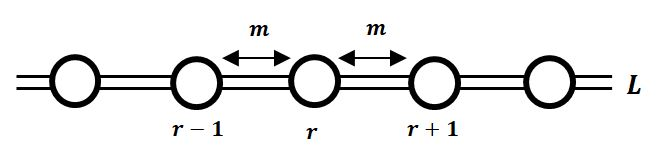
\includegraphics[scale=0.8]{img/model_schematic.JPG}
    \caption{This schematic represents the geographic structure for the model in one dimension. Circles represent demes which are indexed by integer $r$. There are $L$ many demes connected to nearest neighbors via a migration rate $m$. The boundaries are connected to one another, effectively creating a \textit{ring} of demes.}
    \label{fig:schematic}
\end{figure}


Allele frequencies change in each deme over time. We assume that change occurs in discrete generation time. For a single locus with two alleles $a$ and $A$, let $f_r$ be the current allele frequency of $A$ at deme $r$ and time $t$. The allele frequency in this deme at the next generation $f_r'$ is the following:

\begin{equation}
    f_r' = (1-2m-m_\infty)f_r + m(f_{r-1} + f_{r+1}) + m_\infty \bar{f} + \xi_r
\end{equation}


Where $m$ is the symmetric migration rate connecting neighboring demes. $2m$ represents the rate at which individuals in deme $r$ move to the two neighboring demes. $m_\infty$ represents "long range dispersal". Kimura and Weiss (1964) \cite{kimura_stepping_1964} describes this as the rate by which individuals enter new demes as a random sample of the entire population where the probability of sampling $A$ is $\bar{f}$, the frequency of $A$ averaged over each deme. $m_\infty$ is mathematically equivalent to mutation. $\xi_r$ describes random changes in frequency due to genetic drift. As seen in the Wright-Fisher model, $\xi_r$ is a binomial random variable with mean $E[\xi_r]=0$ and $Var[\xi_r] = \frac{f_r(1-f_r)}{N}$ (or $2N$ for a diploid population).


For now, we focus only on migration between nearest neighbors so we ignore $m_\infty$. We also assume $N$ is large in each deme, so that $\xi_r \to 0$. Therefore, we can rearrange terms to arrive at the linear difference equation:

\begin{equation}
    \begin{split}
        f_r' &= (1-2m)f_r + m(f_{r-1} + f_{r+1}) \\ 
        f_r' &= f_r -2mf_r + m(f_{r-1} + f_{r+1}) \\
        f_r' - f_r &= m(f_{r-1} + f_{r+1} - 2f_r)
    \end{split}
\end{equation}


This equation demonstrates the difference in per-generation allele frequency in each deme. We can define $f_r(t+1) = f_r' - f_r$ to arrive at a function describing the per-generation allele frequency change over time and space:

\begin{equation}
    f_r(t+1) = m(f_{r-1} + f_{r+1} -2f_r)
\end{equation}


Note the expected value $E_t[E_r[f_r(t+1)]]$ averaged over position $r$ and time $t$:

\begin{equation} \label{eq:exp_ss}
    \begin{split}
        E_r[f_r(t+1)] &= m(E_r[f_{r-1}] + E_r[f_{r+1}] -2E[f_r]) \\
        &= m(f+f-2f) = 0 \\
        \implies E_t[E_r[f_r(t+1)]] &= 0 
    \end{split}
\end{equation}


On average, migration does not influence the changes in overall allele frequency. 

We can expand the model to two spatial dimensions. This gives an interconnected lattice of demes. Let us only allow for nearest-neighbor migration along cardinal directions, i.e. we allow for individuals in each deme to move along two axes $r$ and $s$:

\begin{figure}[H]
    \centering
    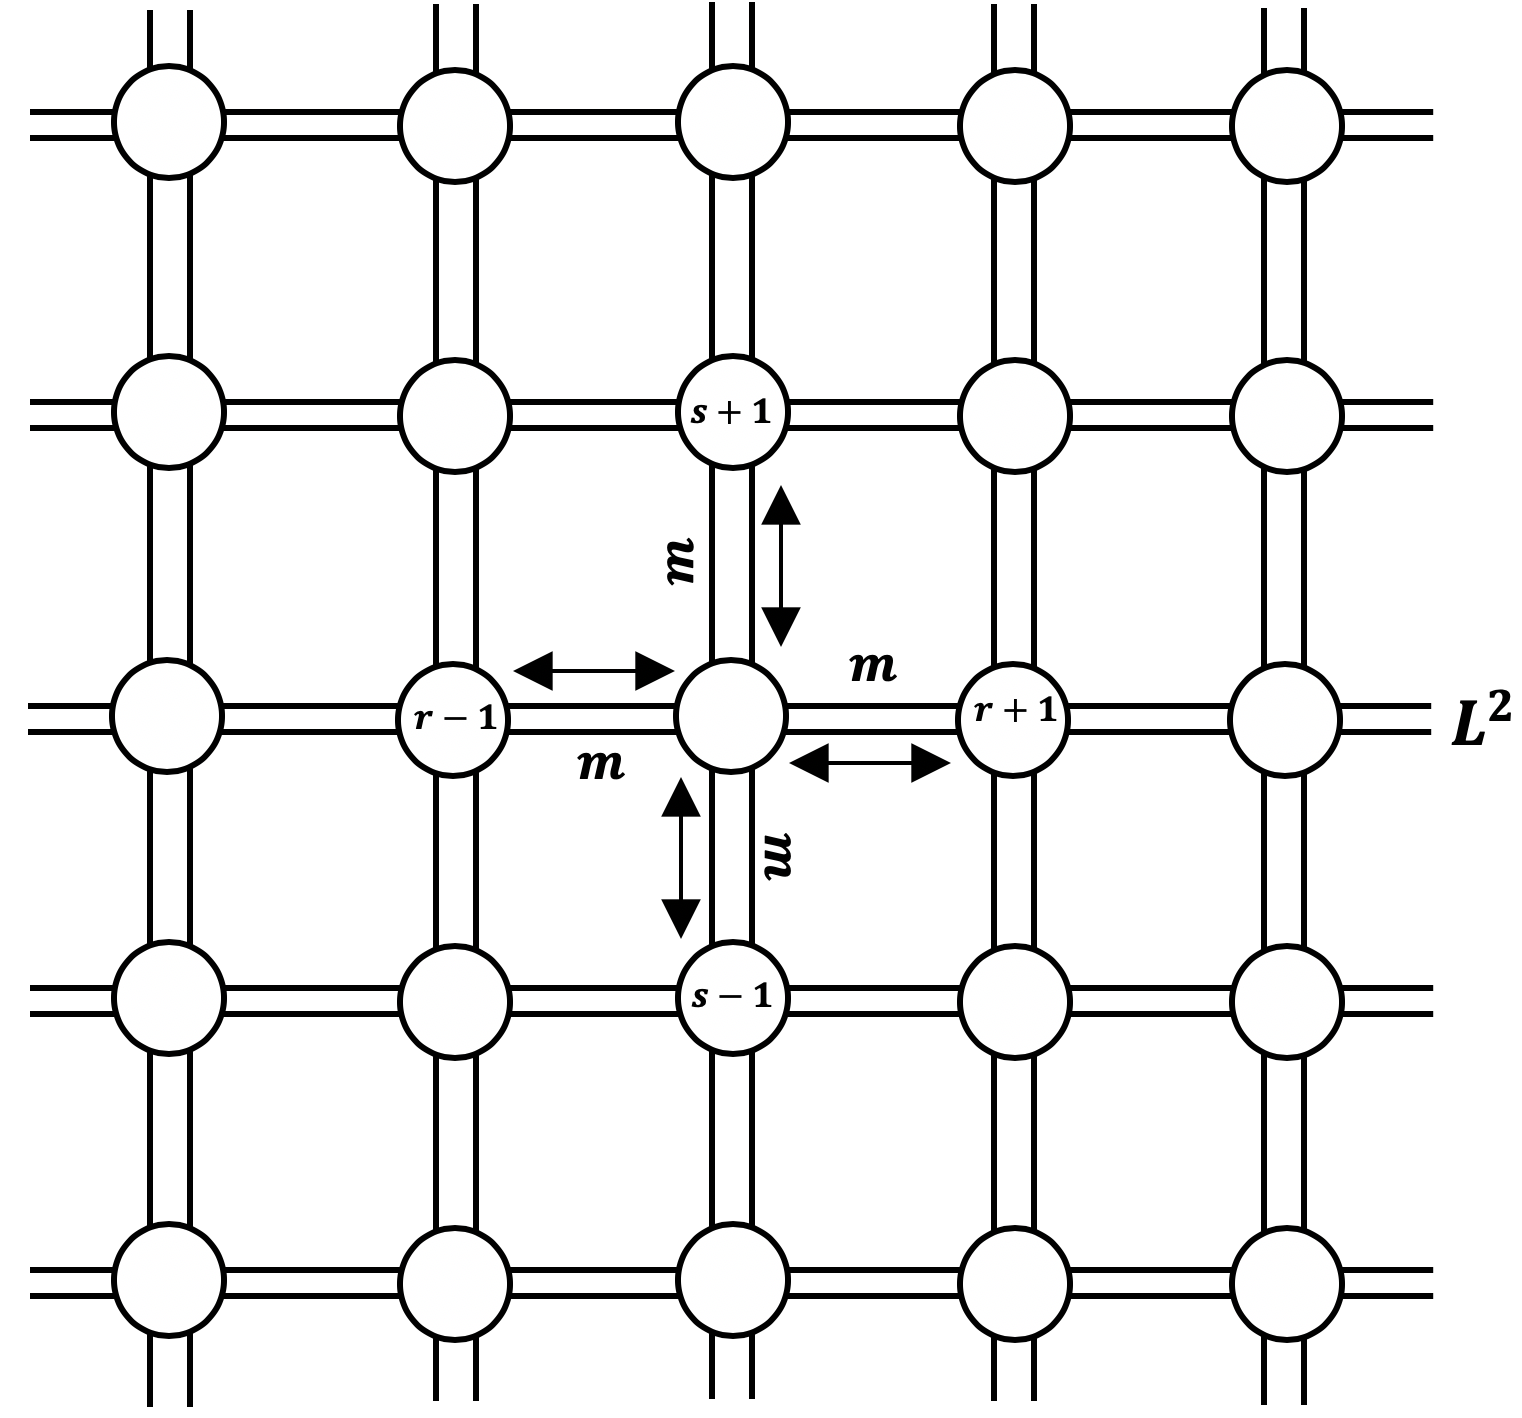
\includegraphics[scale = 0.3]{img/2d_ss.png}
    \caption{The two-dimensional Stepping Stone model with $L^2$ demes. We allow for symmetric migration at rate $m$ between nearest neighbors. Positions on the grid are shown by $r$ along the horizontal axis and $s$ along the vertical axis.}
    \label{fig:2d_ss}
\end{figure}


We can write $f_{r,s}(t+1)$ for the two-dimensional model by simply expanding the form of $f_r(t+1)$ as shown:


\begin{equation} \label{eq:stepstone}
    f_{r,s}(t+1) = m(f_{r-1,s} + f_{r+1,s} + f_{r,s+1} + f_{r,s-1} - 4f_{r,s})
\end{equation}


Note that $E[f] = 0$ in two dimensions as well. The Stepping Stone model provides a useful framework for understanding the influence of migration on evolution. In the next section, we expand upon this framework to incorporate more complex evolutionary forces acting on alleles distributed over the geographic lattice.  


\subsection{The Stepping Stone model with selection} \label{"section:our_model"}

As mentioned previously, our model expands the Stepping Stone model and incorporates natural selection. We describe the allele frequency in a finite population of $N$ individuals grouped into discrete \textit{demes} connected by migration (Figure \ref{fig:schematic}). Each deme is occupied by a fixed, constant population size, which regulates the local population density \cite{felsenstein_pain_1975}. We consider a single genetic locus with two alleles. The focal allele frequency in each deme is $f_r$ with $r$ indexing deme location. Allele frequencies change according to four evolutionary forces:


\begin{enumerate}
    \item \textbf{Mutation} changes one allele to another at rate $\mu$
    \item \textbf{Natural selection} reduces the frequency of the deleterious allele at rate $s$
    \item \textbf{Migration} reduces the allele frequency differences between nearby demes at rate $m$
    \item \textbf{Genetic drift} introduces random noise in a finite population at rate $\frac{1}{N}$, \\ where $N$ is the population size
\end{enumerate}


Recall the $f_r$ describes the current allele frequency at time $t$ and deme $r$. We can write a function of time and space $f_r(t+1)$ and include changes in frequency from selection, mutation, and migration using the rate parameters $s, \mu, m$.

\begin{equation}\label{eq:f_r,t}
    f_r(t+1) = \mu(1-2f_r)-sf_r (1-f_r) + m (f_{r-1}+f_{r+1}-2f_r)
\end{equation}

Note that $f_r(t+1) = \frac{X_r}{N}$. The change in allele count in each deme due to these forces with genetic drift $X_r(t+1) | \hat{f}(t)$ is described by the equation:

\begin{equation}
    \label{eq:model}
    X_r(t+1) | \hat{f}(t) \sim Binom(N,f_r(t+1))
\end{equation}


$\hat{f}(t)$ describes the allele frequency at time $t$ across the spatial environment. Note that we consider a symmetric migration rate. The rate at which individuals leave their current deme is the same as the rate at which individuals enter that deme. We also consider a symmetric mutation rate. The rate at which allele $a$ changes into $A$ is the same as the reverse mutation. Loci are modeled as independent replicates.

While these models have been studied extensively \cite{felsenstein_genetic_1975}\cite{malecot_heterozygosity_1975}\cite{sawyer_branching_1976}, most work has been focused on neutral evolution. A caveat to this is the study of "clines", or measurable gradients of biological characteristics across geographic ranges. Some population geneticists and evolutionary biologists have studied changes in clines in situations of non-neutral evolution. \cite{baines_role_2004} Still, many of these studies still focus on examining the influence of genetic drift on cline patterns. \cite{polechova_genetic_2011} The main difference between the theory of clines and the non-neutral evolutionary theory we propose, is that cline theory is concerned with the \textit{mean} allele frequency, while we are concerned with the \textit{distribution} of allele frequencies.\cite{vasemagi_adaptive_2006} This distribution is more relevant for rare alleles and large samples. 


Expanding the Wright-Fisher model allows us to examine allele frequencies acted upon by each of the four evolutionary forces. We simulate the evolution of rare deleterious alleles over many generations and over large geographic environments. Using this equation, important information about the evolution of rare deleterious alleles can be discovered. In the next chapter, we will derive important quantities that describe the average number of rare allele copies as a function of the evolutionary parameters along with the quantity describing the average geographic range of an allele. We will also describe the expected distribution of allele frequencies across demes, known as the \textit{Site Frequency Spectrum} (SFS).

The SFS is an observed quantity summarizing the distribution of allele frequencies in a population \cite{lapierre_accuracy_2017}. It is essentially a histogram illustrating the number of alleles at different loci that exist at certain frequencies in the population. In a well-mixed population with neutral mutations, there is a power-law showing most mutations existing at low frequencies with fewer mutations at high frequencies. Deleterious mutations rarely reach high frequencies, and the SFS of deleterious alleles reflects this.

\begin{figure}[H]
    \centering
    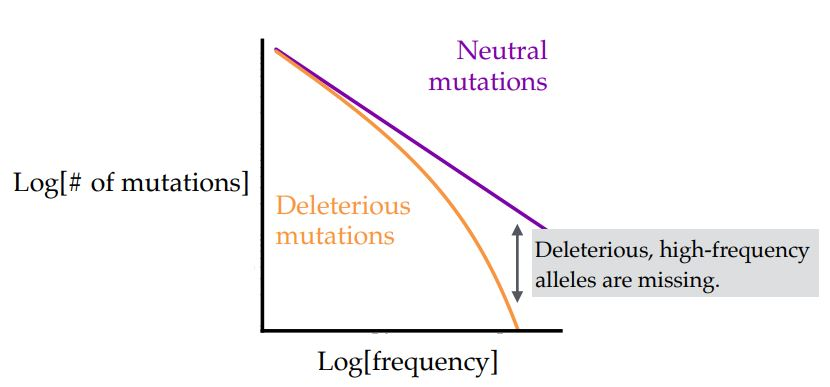
\includegraphics[scale=0.7]{img/sfs_schematic.JPG}
    \caption{This schematic illustrates the SFS for neutral and deleterious mutations in a well-mixed population. Deleterious mutations exist mostly at low frequencies.}
    \label{fig:sfs_schema}
\end{figure}


Our approach involves first simulating the underlying distribution of allele frequencies, and second, sampling from this distribution using a variety of sampling scheme. Our subsequent analysis examines the information loss as a function of sampling. We are interested in the interaction between the process of sampling and the "unobserved" underlying frequency distribution. 

\begin{figure}[H]
    \centering
    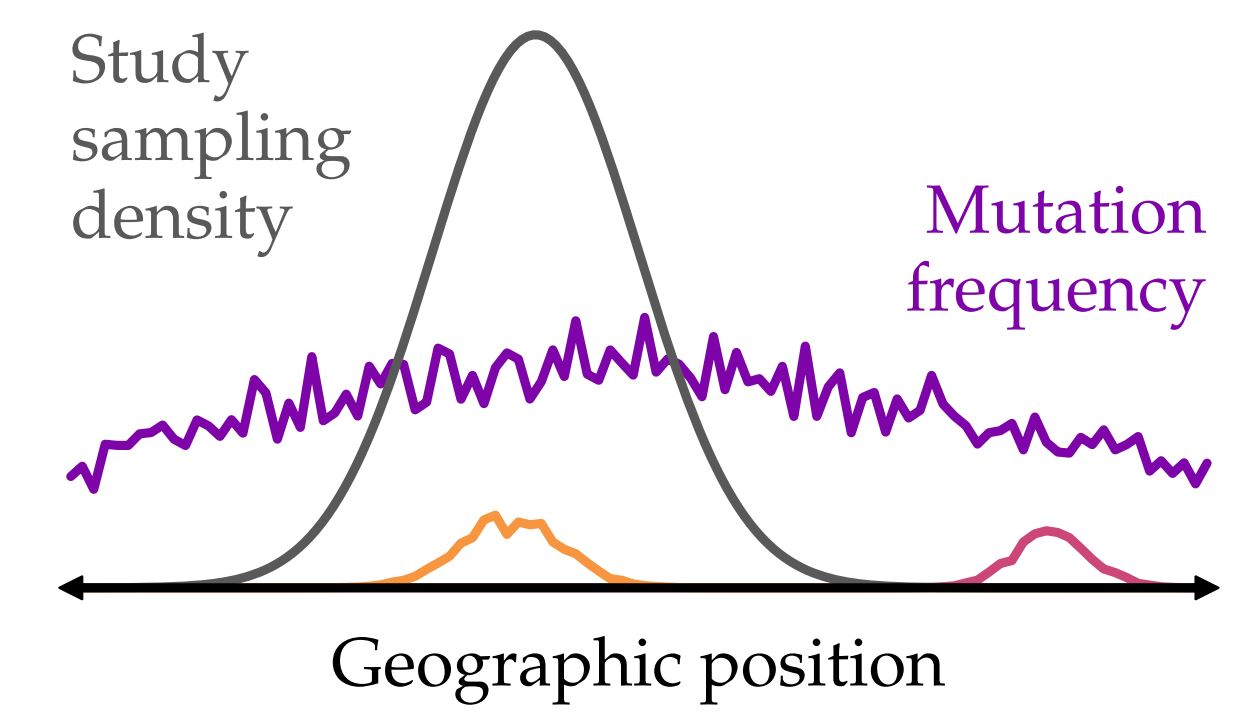
\includegraphics[scale=0.35]{img/smapling_schematic.JPG}
    \caption{This schematic illustrates the interaction between the underlying allele frequency distribution and the sampling scheme imposed by an association study. We see that alleles are typically confined to a range of geographic positions, with rare alleles having a smaller range. We expect the distribution of alleles observed in a GWAS to depend on the location of the sampling distribution relative to the allele frequency distribution.}
    \label{fig:sampling_schematic}
\end{figure}

\newpage
\section{Simulations}

This section describes the various tools used to simulate our model. In theory-based research, simulations are important for several reasons. First, they allow us to observe a system that is typically too complex to study empirically. Simulations allow us to study evolution over thousands of generations in a matter of seconds. Second, simulations allow us to validate theoretical predictions made by our model. We can derive properties of our system analytically, and show that these properties hold computationally. Much of our project results come from first making predictions based on our model, and then confirming these predictions with simulations. Hundreds of simulations have been run throughout the course of this project, producing hundreds of gigabytes of data. The University of Chicago Research Computing Cluster has made this process possible. All code presented in this section is available at github.com/chrisporras/spatial\_simulations. 


Our simulations were designed using \code{NumPy} arrays and custom-written functions in \code{Python}. \code{NumPy} ("\textbf{Num}erical \textbf{Py}thon extensions") is the staple \code{Python} package for working with large sets of numerical data. The package demonstrates superior computational efficiency, both in terms of processing speed and memory usage. \code{NumPy} is at the core of much scientific computing.\cite{van_der_walt_numpy_2011} We use the package to efficiently create, manipulate, and store arrays of simulation data. The following sections demonstrate our process. 


\subsection{Evolution in discrete time and space}

Recall that our model describes the change in allele frequencies per generation in discrete demes connected by migration:

\begin{equation}
    \tag{\ref{eq:model} revisited}
    X_r(t+1) | \hat{f}(t) \sim Binom(N,f_r(t+1))
\end{equation}

Where $f_r(t+1)$ is given by:

\begin{equation}
    \tag{\ref{eq:f_r,t} revisited}
    f_r(t+1) = \mu(1-2f_r)-sf_r (1-f_r) + m (f_{r-1}+f_{r+1}-2f_r)
\end{equation}

Our simulations use this equation to generate changes in allele frequencies over time, given an initial allele frequency $f_0 = \frac{1}{N}$ and a set of population parameters. We begin with a one deme population ($L = 1$) and the following parameters:

\lstinputlisting[language=iPython, caption = Population parameters, label = code:params]{src/param_list.py} 

Our simulation output contains a vector of allele frequency values for every generation. We perform many independent replicates of each trajectory to represent multiple loci and compute statistics from our data. The figure below shows an example stochastic trajectory of allele frequencies over time. With purifying natural selection (large $s$), the allele remains rare as $s$ determines the rate at which the allele is removed from the population. We observe this to be the case in the example shown.


\begin{figure}[H]
    \centering
    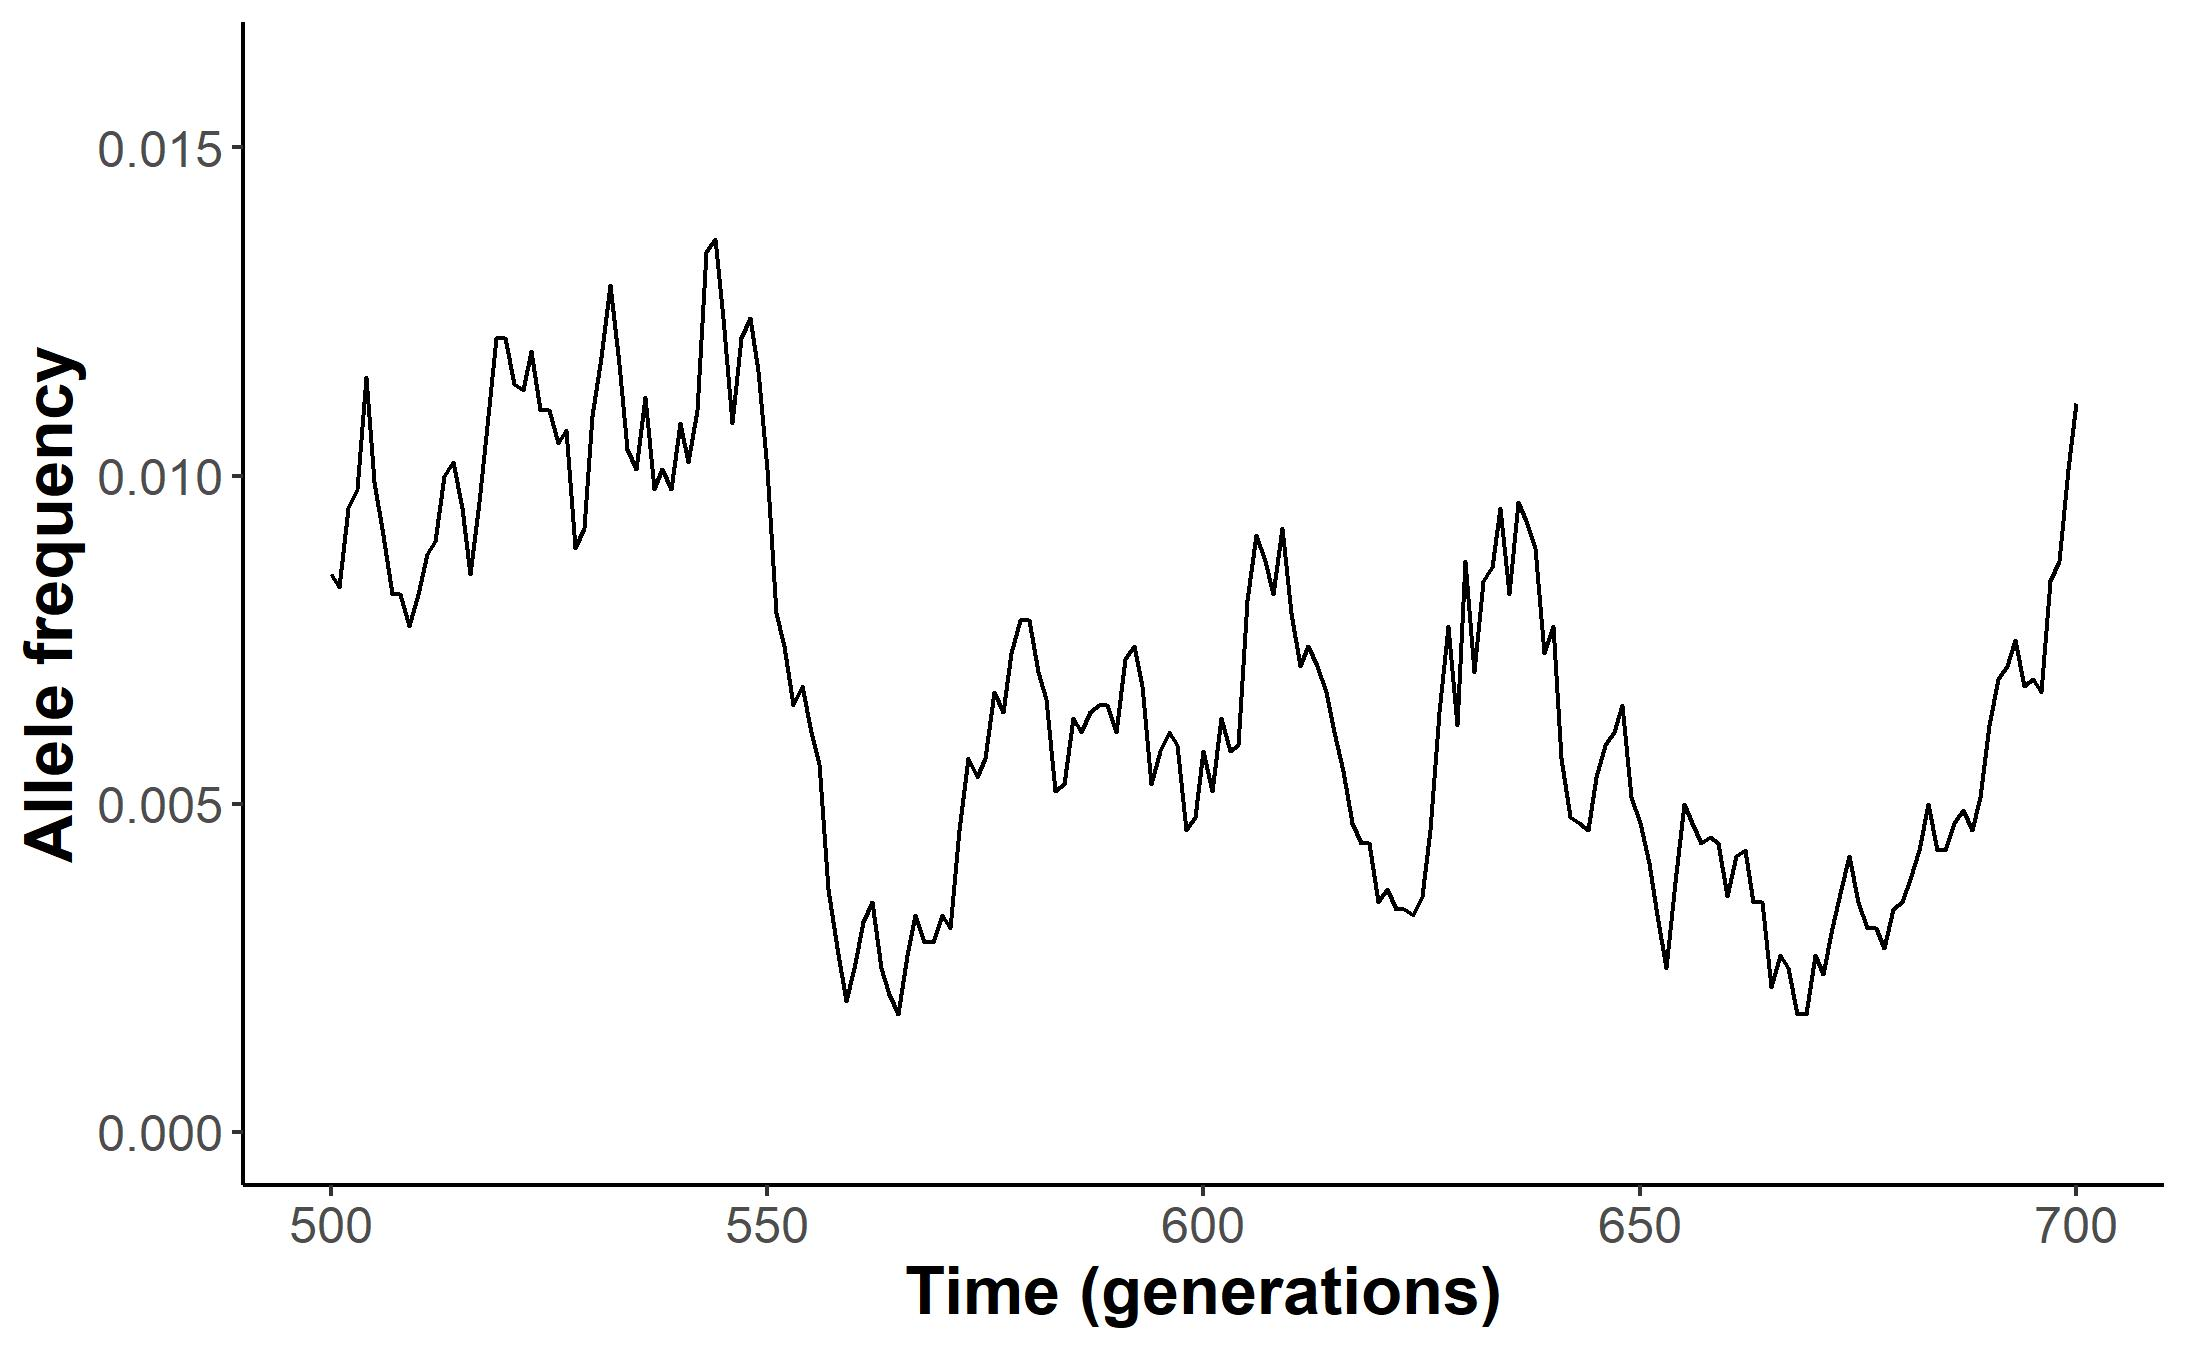
\includegraphics[scale=0.5]{img/time_series.jpg}
    \caption{An example simulation output plot of allele frequencies changing over time.}
    \label{fig:time_series}
\end{figure}


As mentioned, \code{NumPy} allows us to efficiently run simulations of our model. We can define a \code{SS\_WF\_sim()} function to accept our population parameters and calculate $df$ given by equation (\ref{eq:model}). We perform this calculation for every generation, storing a matrix $\bf{f}$ containing allele frequencies over time at each deme. Stochasticity is incorporated into our population using \code{NumPy} random number generators. We store these matrices as \code{.npy} \textit{byte} files which save on storage space and allow other \code{NumPy} programs to quickly load in our data. The script used to perform our simulations is shown below:

\lstinputlisting[language=iPython, caption = Python script used to simulate Wright-Fisher + Stepping Stone model]{src/python_ss_wf.py}

This script is much more concise than our \code{SLiM} script (Supplement section \ref{section:slim}) and offers computation speed that is orders of magnitude faster. We use \code{np.random.binomial()} to generate binomial random samples given probability $p = f_{t-1} + df$. This simulates genetic drift through the manner described in section  \ref{section:neutral_wf}. What may be less clear is our use of \code{laplace()} from the \code{SciPy} package \cite{scipy} to incorporate migration. In mathematical terms, the \code{laplace()} function computes the discrete \textit{Laplacian} of our frequency matrix $\textbf{f}$ and performs a \text{convolution} of our matrix with its Laplacian. The Laplacian of a discrete-valued function $\psi(x,y)$ (written $\nabla^2 \psi(x,y)$) is defined as the following:

\begin{equation}
    \nabla^2 \psi(x,y) =  \frac{1}{h^2}(\psi_{x+h,y} + \psi_{x-h,y} + \psi_{x,y+h} + \psi_{x,y-h} - 4\psi_{x,y})
\end{equation}

When we set $h = 1$, $\psi(x,y) = \frac{df}{dt}(r,s)$ and multiply by migration rate $m$, we arrive at our equation for migration dynamics in the two-dimensional Stepping Stone model:

\begin{equation} 
    \tag{\ref{eq:stepstone} revisited}
    m[\nabla^2 f_{r,s}(t+1)] = m(f_{r-1,s} + f_{r+1,s} + f_{r,s+1} + f_{r,s-1} - 4f_{r,s})
\end{equation}


Note that we specify \code{mode} = "wrap" for the \code{lapace()} function. This computes the discrete Laplacian for periodic boundary conditions, which we use to capture the connected boundaries of the Stepping Stone model. The \code{laplace()} generalizes our simulation to as many spatial dimensions as specified in the \code{dims} parameter. We use the exact same script to simulate Stepping Stone migration in both one and two dimensional models. When we call the \code{laplace()} function on our matrix $\text{bf}$, the calculation in equation \ref{eq:stepstone} is performed across all pairs of $(r,s)$ neighbor demes and $df$ is computed accordingly. All this is done in a computationally efficient, generalized fashion.


We perform many replicate simulations over various combinations of population parameters. Because our simulations are stochastic, we need many replicates to compute useful statistics and relate our theoretical predictions to our generated data. Our goal is essentially to explore how changing the aforementioned population parameters influences what we see in our simulations. 


\subsection{Simulated sampling}
This section describes our method for simulating the sampling process inherent in GWAS. Recall that we are interested in the interaction between the underlying distribution of allele frequencies and the distribution of frequencies observed in a population sample (Figure: \ref{fig:sampling_schematic}). We expect the ability to detect alleles in a GWAS sample to depend on the population parameters (particularly the rates of selection and migration) and on the strategy used to select members of a GWAS corhort. Geography plays a key role in the search of rare disease-causing alleles. Intuitively, \texit{where} researchers sample individuals from and \textit{how many} individuals are sampled from each location determines which alleles are detectable.


Essentially, we want to randomly draw alleles from our simulated population according to some sampling probability distribution. The probabililty of sampling an allele at deme $r$ depends on the frequency of that allele across each location $\hat{f}(t)$ and the probability that a sample is taken from each deme. We accomplish this by computing a \textit{convolution} with our allele frequency matrix $\textbf{f}$. A convolution of discrete-valued functions $f$ and $g$ is defined as:

\begin{equation}\label{eq:convolution}
    F(r) = (f*g)(r) = \sum_{d=0}^L f(r)g(r-d)
\end{equation}


Where $f$ and $g$ are both functions of $r$, the convolution expresses how $g$ changes the shape of $f$ over all $g(r)$. For our model, we assume a Gaussian sampling distribution $g(r)$ with a fixed center at deme $\hat{r}$ and a specified standard deviation, or width, $w$. We average over all possible relative sampling positions. The convolution allows us to compute the average probability of sampling the allele over all possible centers $\hat{r}$. The output of this calculation is another matrix of sampled allele frequencies $\bf{F}$ that is of the same dimensions as $\bf{f}$. The following code snippet shows our implementation of this process using the \code{SciPy} Gaussian convolution filter. 


\lstinputlisting[language=iPython, caption = Python script to implement sampling process]{src/sample.py}


We can now add $w$ to our list of simulation parameters. We see in figure \ref{fig:sampling_w} that increasing $w$ flattens out the distribution of allele frequencies seen in a one-dimensional spatial model. The broader our sampling width, the harder it is to detect rare, localized alleles. Our results primarily focus on exploring the relationships between our population parameters. Altering our parameters changes the allele frequency trajectories observed, providing insight into how the evolutionary process and the sampling process influence allele detection.    

\begin{figure}[H]
    \centering
    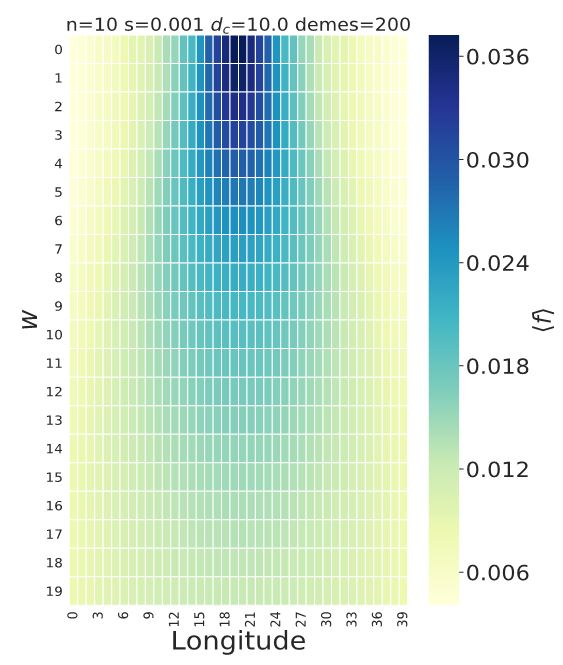
\includegraphics[scale=0.8]{img/sampling_heatmap.JPG}
    \caption{Increasing $w$ smooths the spatial distribution of allele frequencies. An allele that exists mostly at the center of the one-dimensional simulation is undetectable at broad sampling widths.}
    \label{fig:sampling_w}
\end{figure}


%% End with mentioning Snakemake?